% Setup - do not change
\documentclass[11pt]{article}
\usepackage[top=0.9in, left=0.9in, bottom=0.9in, right=0.9in]{geometry} 
\usepackage{parskip}

\usepackage[english]{babel}
\usepackage[utf8]{inputenc}
\usepackage{amsmath,amsthm,amssymb,graphicx,pdfpages,lipsum,hyperref}
\usepackage[none]{hyphenat}
\usepackage{csquotes}

\setlength\parindent{0pt}
%%%%%%%%%%%%%%%%%%%%%%%%%%%%%%%%%%%%%%%%%%%%%%%%%%%%%%%%%%%%%%%%%%%
% add other packages here if required

\usepackage[export]{adjustbox}

%% Bibliography are specified in this file. You can also choose inline bib style if you want to. But make sure your citation style is consistent (and proper)
% For more details on citation: https://library.unimelb.edu.au/recite
\usepackage[sorting = none]{biblatex}
\addbibresource{references.bib}

%%%%%%%%%%%%%%%%%%%%%%%%%%%%%%%%%%%%%%%%%%%%%%%%%%%%%%%%%%%%%%%%%%% the '%' symbol denotes comments

% Begin document creation
% DELETE THE \lipsum PLACEHOLDERS WHEN YOU BEGIN
\title{\textbf{Applied Data Science (MAST30034) Project 1: Quantitative Analysis} \\ Quantitative Analysis Of The New York City Taxi Data}
\author{
Insert Student Name \\
Student ID: XXXXXX \\
%% Replace the link with your github repo
% 1. Remember to escape underscore in the link.
% 2. Remember to include the commit you want to submit in the link
\href{https://github.com/MAST30034-Applied-Data-Science/mast30034\_p1\_template/tree/fd9f1dd17fdbcb5b119b70c93a22da8210d44fd7}{Github repo with commit}
}

\begin{document}
\maketitle

\section{Introduction}
% Link to a 30 min tutorial if you require revision: https://www.overleaf.com/learn/latex/Learn_LaTeX_in_30_minutes

When we talk about the symbols of the New York, you might think the Statue of Liberty. But one thing that also is the symbols of the New York city is taxi. There are two varieties taxicabs yellow and green in New York City. They have same fare structure. The difference is that the yellow one can pick up passengers anywhere in the five boroughs, while the green one can pick up passengers in Upper Manhattan, the Bronx, Brooklyn, Queens and Staten Island.  The New York City Taxi and Limousine Commission (TLC) a private companies that license the taxi operate.\cite{Taxis}.
The only vehicles that can pick up passengers anywhere in New York City is the taxi. Each taxi must have a medallion affixed to it by law.\cite{YellowCab}. Taxis are comfy, they are available all the time, It is important for us to find out the how weather effect the New York City taxi business.  


% You can have \section{}, \subsection{}, and \subsubsection{}
\section{EDA}

\subsection{Load Data}

\subsubsection{Yellow Taxi Trip Records, weather and Taxi Zone data}
The Yellow Taxi Trip Records data we use is in the year 2019 January April, July, and October yellow taxi trip data in New York City. Since these 4 months represent the four seasons of the New York City. Which can use for weather analysis. The data is provided in New York City Taxi and Limousine Commission.

The weather data I use is from kaggle New York City Weather Data 2019.This dataset was gathered to be used in the Big Data Derby 2022 competition. However, it can obviously be used for any other purposes. Horses are affected by weather conditions, so knowing the day's temperature, snowfall, precipitation, etc will definitely be useful.Weather data collected from the National Weather Service. The data collects in 2019 all days weather data, include each day the minimum temperature(measured in Fahrenheit), maximum temperature(measured in Fahrenheit), average temperature(measured in Fahrenheit), precipitation(measured in inches), new snow fall(measured in inches), and current snow depth.\cite{kaggle}

The Taxi zone data \cite{TaxiZone}. By using this data we can get where the taxi in New York City, combine with the Taxi Zone Look Up Table file we can draw a map in New York City.

\subsection{Preprocess Data}

It approximately got 28696876 trip records for 2019 year 4 months data set with 19 columns of attributes. The data takes 4.1G memory. By changing the datatypes we reduce the data memory usage.

\subsubsection{Clean Data}

First thing we check is the missing data. Yellow taxi data set  missing value is list below:
151810 values are missing for passenger\_count, RatecodeID, store\_and\_fwd\_flag features. 5008025 missing values for the congestion\_surcharge feature. According to the feature context, I am able to filter out some error like the distance can't be negative. Finally, the PULocationID and DOLocationID should within NYC taxi zone.\cite{TaxiZone}


Next, in figure \ref{fig:image1} and in figure \ref{fig:image2},we plot the data distribution.

\begin{figure}[!h]
    % change the scale multiplier to make the figures smaller or larger
    \centering
    \adjincludegraphics[height=7cm,clip]{plots/p1.png}
    % \includegraphics[width=\textwidth]{download.png}
    % this ensures your figures are centered where possible
    \caption{trip distance distribution} % refer to this image as (Figure 1)
    \label{fig:image1}
\end{figure}

\begin{figure}[!h]
    % change the scale multiplier to make the figures smaller or larger
    \centering
    \adjincludegraphics[height=7cm,clip]{plots/p2.png}
    % \includegraphics[width=\textwidth]{download.png}
    % this ensures your figures are centered where possible
    \caption{total amount distribution} % refer to this image as (Figure 1)
    \label{fig:image2}
\end{figure}

\subsubsection{Create Feature}

The difference between pickup and drop-off time is a useful information for us to know the  period of each trip. The features: tpep\_pickup\_datetime, tpep\_dropoff\_datetime, store\_and\_fwd\_flag that are no longer the features we needed. Finally, I select the date in the 4 months of both taxi and weather dataset.

\subsection{Visualisation}
\subsubsection{Map}

These 4 months the total amount of activity in New York City is show. In figure \ref{fig:image3}, The brighter and yellow regions indicate that there are exits more taxi activity. In Manhattan it got most pickups and drop-off activities.

\begin{figure}[!h]
    % change the scale multiplier to make the figures smaller or larger
    \centering
    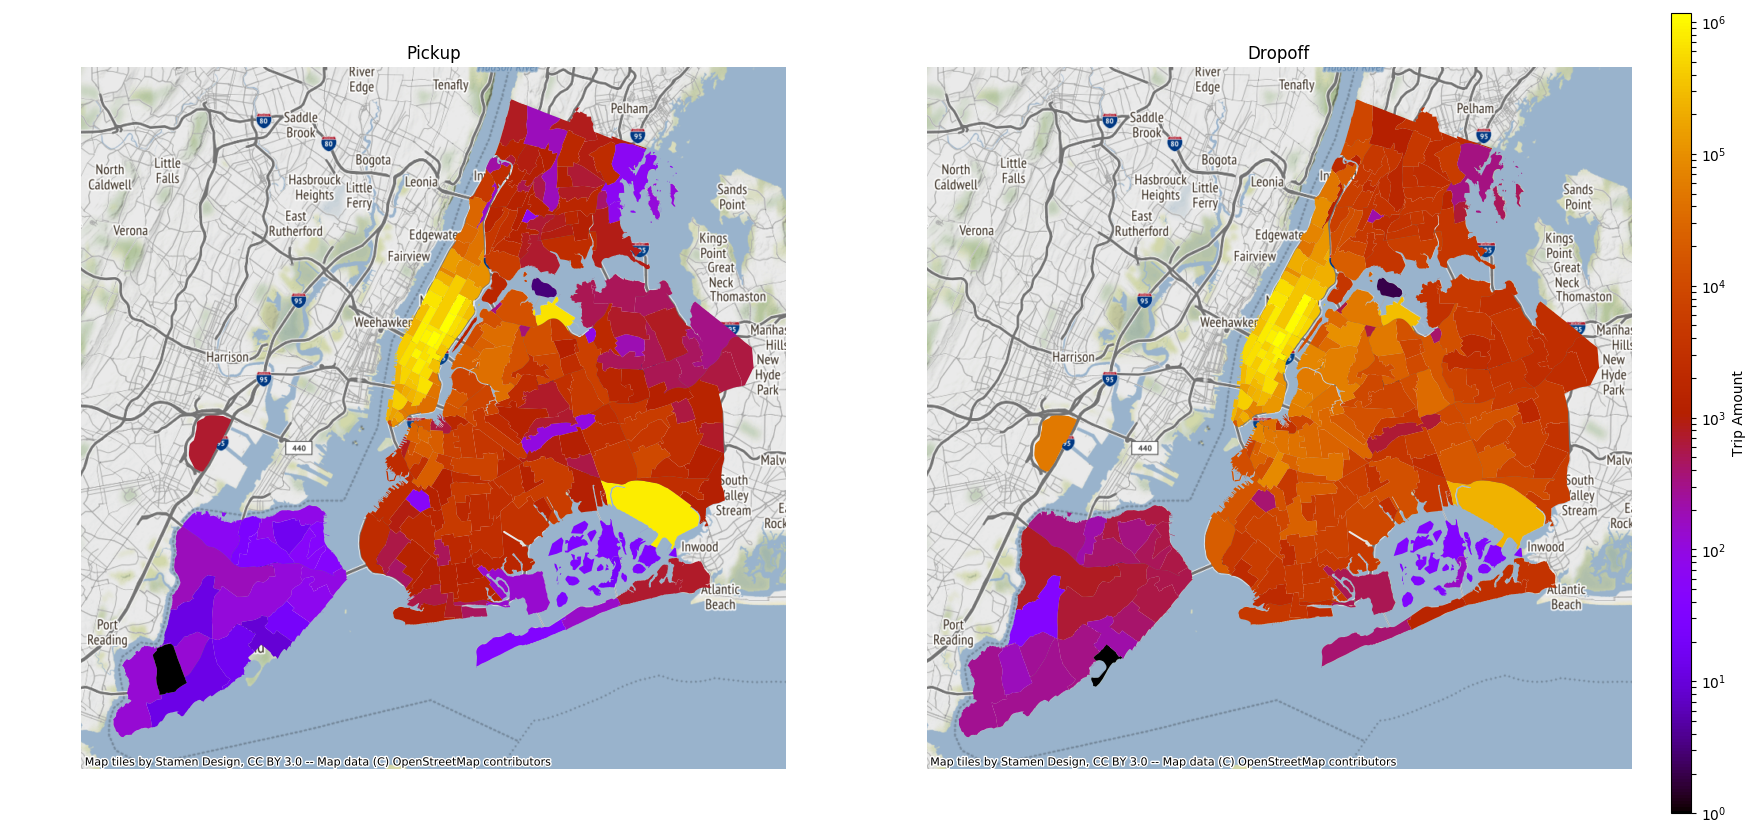
\includegraphics[width=0.8\textwidth]{plots/p3.png}
    % \includegraphics[width=\textwidth]{download.png}
    % this ensures your figures are centered where possible
    \caption{Taxi Pickup Frequency} % refer to this image as (Figure 1)
    \label{fig:image2}
\end{figure}

\subsubsection{Weather Impact}
In this section we investigate how weather affects the taxi business. The following scatter plots shows the weather Average temperature of the day in F versus different data features like:


'passenger\_count','trip\_distance','tip\_amount','total\_amount' 'period'. 

\begin{figure}[!h]
    % change the scale multiplier to make the figures smaller or larger
    \centering
    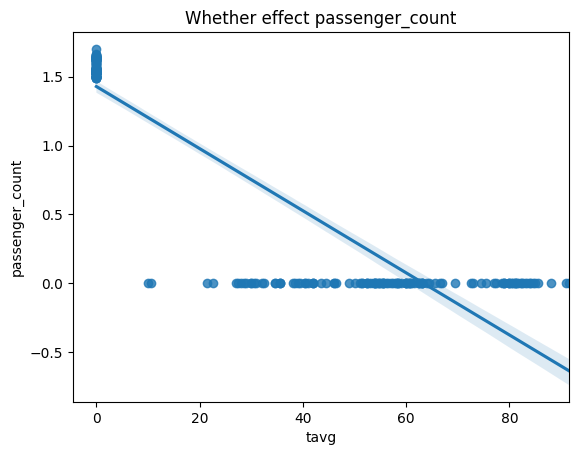
\includegraphics[width=0.5\textwidth]{plots/p4.png}
    % \includegraphics[width=\textwidth]{download.png}
    % this ensures your figures are centered where possible
    \caption{Weather Impact passenger count} % refer to this image as (Figure 1)
    \label{fig:image3}
\end{figure}

\begin{figure}[!h]
    % change the scale multiplier to make the figures smaller or larger
    \centering
    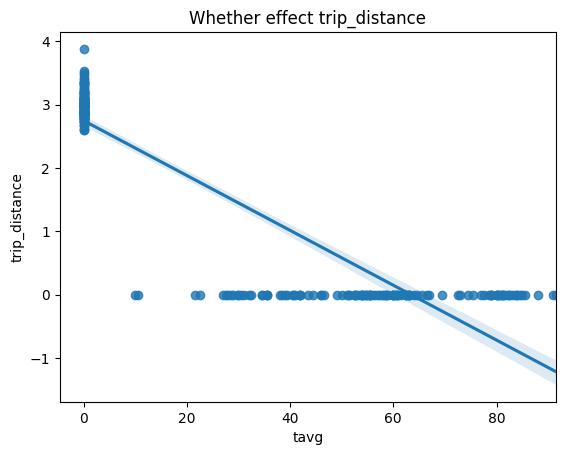
\includegraphics[width=0.5\textwidth]{plots/p5.png}
    % \includegraphics[width=\textwidth]{download.png}
    % this ensures your figures are centered where possible
    \caption{Weather Impact trip distance} % refer to this image as (Figure 1)
    \label{fig:image3}
\end{figure}

\begin{figure}[!h]
    % change the scale multiplier to make the figures smaller or larger
    \centering
    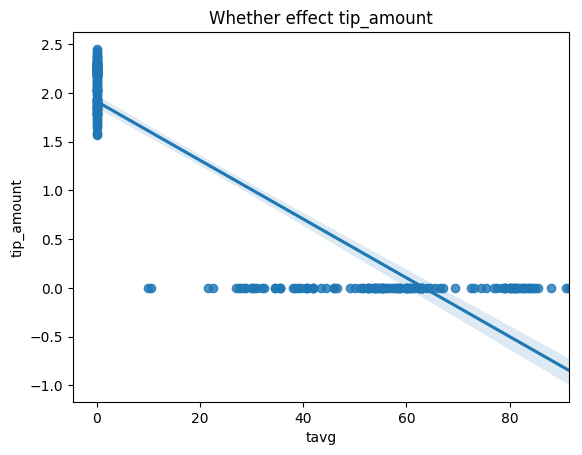
\includegraphics[width=0.5\textwidth]{plots/p6.png}
    % \includegraphics[width=\textwidth]{download.png}
    % this ensures your figures are centered where possible
    \caption{Weather Impact tip amount} % refer to this image as (Figure 1)
    \label{fig:image3}
\end{figure}


\begin{figure}[!h]
    % change the scale multiplier to make the figures smaller or larger
    \centering
    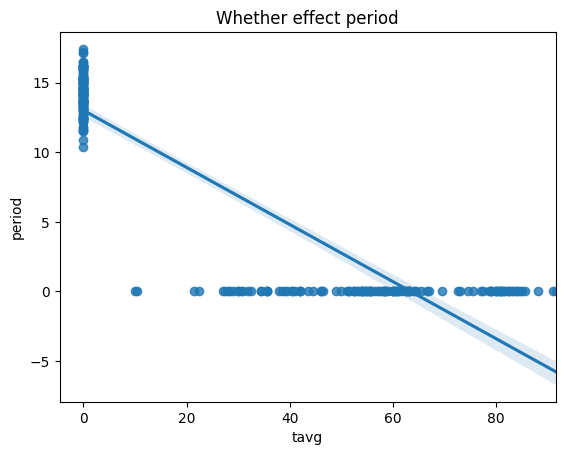
\includegraphics[width=0.5\textwidth]{plots/p7.png}
    % \includegraphics[width=\textwidth]{download.png}
    % this ensures your figures are centered where possible
    \caption{Weather Impact period} % refer to this image as (Figure 1)
    \label{fig:image3}
\end{figure}

\begin{figure}[!h]
    % change the scale multiplier to make the figures smaller or larger
    \centering
    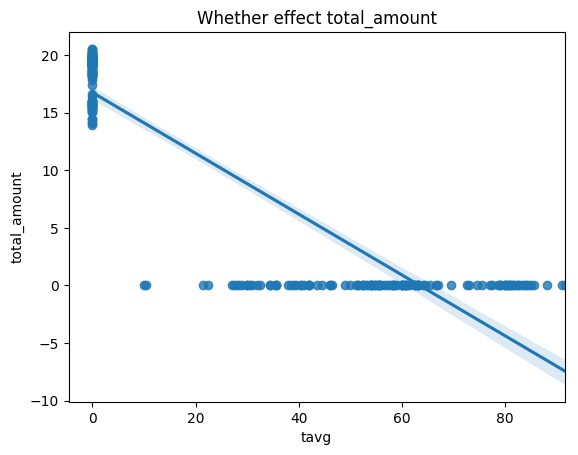
\includegraphics[width=0.5\textwidth]{plots/p8.png}
    % \includegraphics[width=\textwidth]{download.png}
    % this ensures your figures are centered where possible
    \caption{Weather Impact total amount} % refer to this image as (Figure 1)
    \label{fig:image3}
\end{figure}

From figure \ref{fig:image3} , We can draw the conclusion that the taxi bussiness get more tip and trip distance when the weather gets cold.

\subsubsection{Season affect}
In this section we shows that how the seasons affect the taxi bussiness. 
As shown in figure \ref{fig:image4}, The trip distance, tip amount doesn't change much through the seasons. The period and total amount get decrease in winter compare to the other seasons. 

\begin{figure}[!h]
    % change the scale multiplier to make the figures smaller or larger
    \centering
    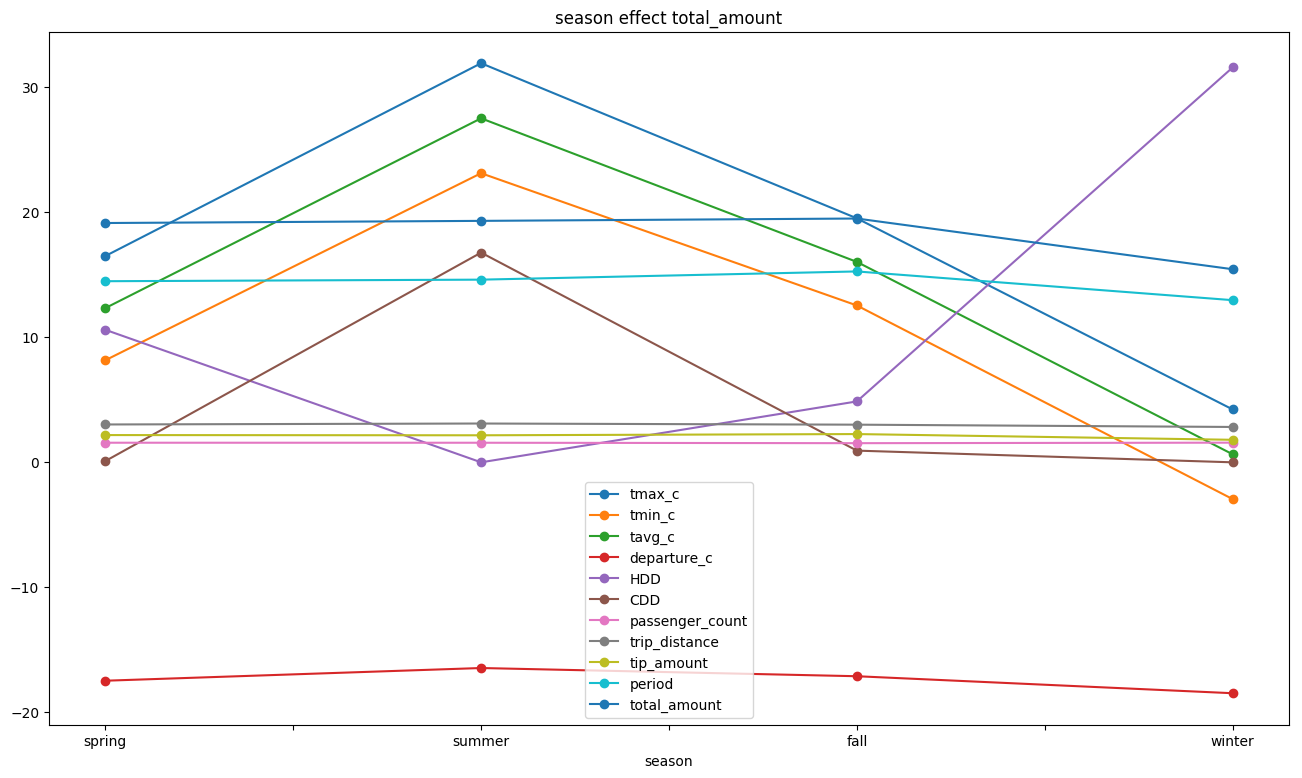
\includegraphics[width=0.8\textwidth]{plots/p9.png}
    % \includegraphics[width=\textwidth]{download.png}
    % this ensures your figures are centered where possible
    \caption{Season affect} % refer to this image as (Figure 1)
    \label{fig:image4}
\end{figure}


\section{Modelling}

In Modeling section we want to see which features contribute to the total\_amount feature. Since the total\_amount is the most important for taxi driver.

\subsection{Correlation}
The correlation heat map about data features shown in figure \ref{fig:image9}, the features like 'trip\_distance', 'fare\_amount', 'tip\_amount', 'tolls\_amount', 'period' get high correlation scores of the total\_amount.

\begin{figure}[!h]
    % change the scale multiplier to make the figures smaller or larger
    \centering
    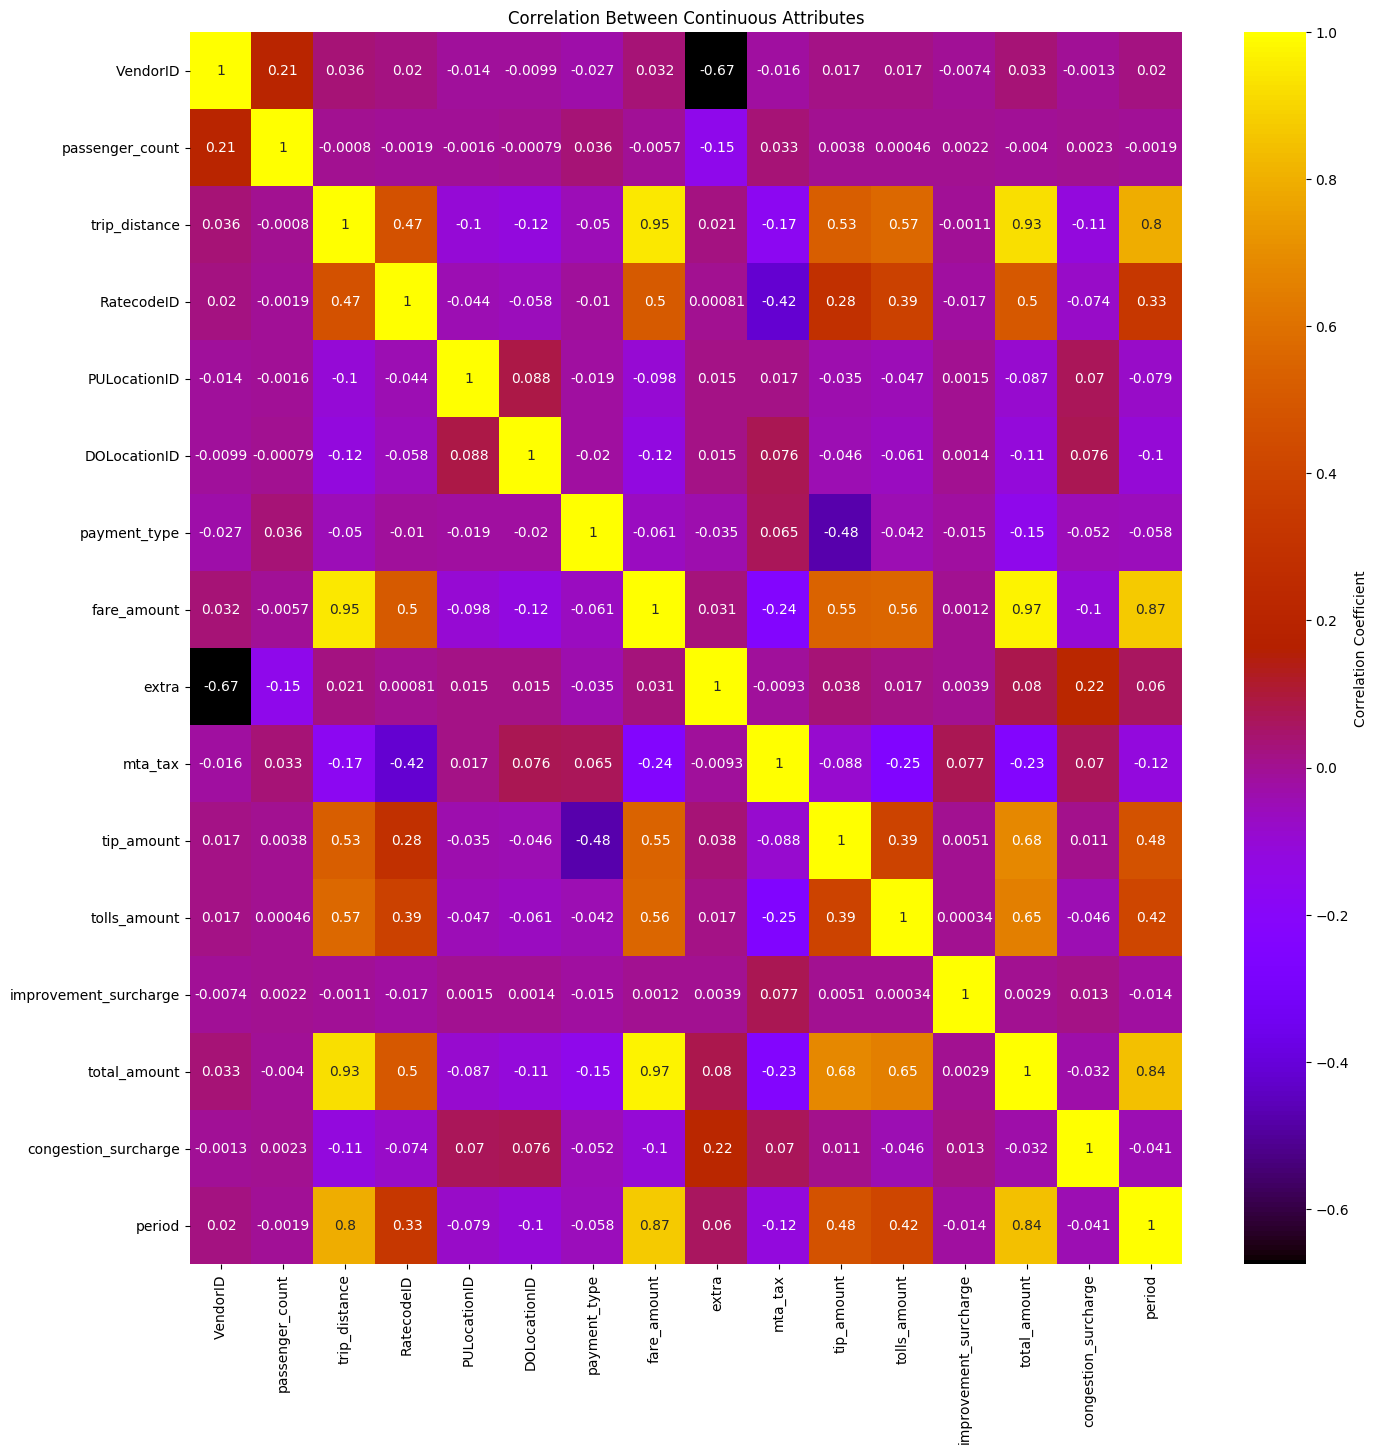
\includegraphics[width=0.8\textwidth]{plots/p10.png}
    % \includegraphics[width=\textwidth]{download.png}
    % this ensures your figures are centered where possible
    \caption{Correlation Coefficient} % refer to this image as (Figure 1)
    \label{fig:image9}
\end{figure}

\subsection{regression model}
The  total\_amount data feature will be predict using three regression models. They are linear regression model, Ridge regression model and Lasso regression model. According to the correlation heat map we created. We use feature 'trip\_distance', 'fare\_amount', 'tip\_amount', 'tolls\_amount', 'period' as our X feature. The y is of course the total\_amount.  The train-test split method is used to randomly split sampled data into 70\% training set and 30\% testing set.

\subsection{Evaluation & Results}

When we create model, we need to know how well it perform. The evaluation step is for us to know how well the model perform.
By using Root Mean Square Error and R2 score. We get a general idea about how well the model is perform. In the table\ref{table1}, we can see that all model perform the same.

\begin{table}[h]
    \centering  
    \caption{result table}  
    \label{table1} 
    %字母的个数对应列数,|代表分割线
    % l代表左对齐,c代表居中,r代表右对齐
    \begin{tabular}{|c|c|c|c|c|}  
        \hline  % 表格的横线
        & & & & \\[-6pt]  %可以避免文字偏上来调整文字与上边界的距离
        Model&Train RMSE&Test RMSE&Train R2&Test R2 \\  % 表格中的内容,用&分开,\\表示下一行
        \hline
        & & & & \\[-6pt]  %可以避免文字偏上 
        Linear&1.25&1.25&1.0& 1.0 \\
        Ridge&1.25&1.25&1.0& 1.0 \\
        Lasso&1.25&1.25&1.0& 1.0 \\
        \hline
    \end{tabular}
\end{table}

The coefficient of the three models are show:

\begin{figure}[!h]
    % change the scale multiplier to make the figures smaller or larger
    \centering
    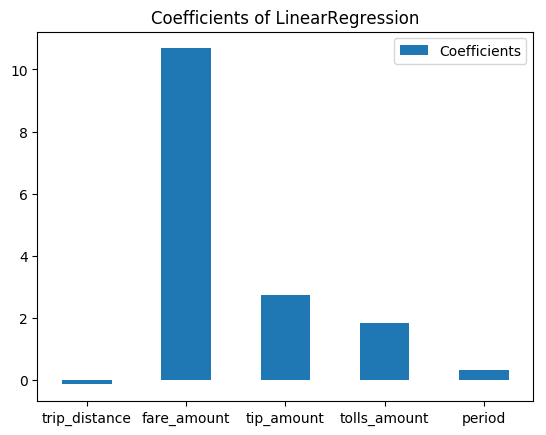
\includegraphics[width=0.7\textwidth]{plots/p11.png}
    % \includegraphics[width=\textwidth]{download.png}
    % this ensures your figures are centered where possible
    \caption{Linear} % refer to this image as (Figure 1)
    \label{fig:image4}
\end{figure}


\begin{figure}[!h]
    % change the scale multiplier to make the figures smaller or larger
    \centering
    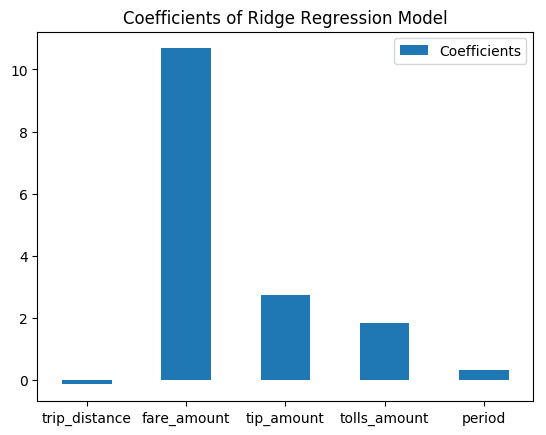
\includegraphics[width=0.7\textwidth]{plots/p12.png}
    % \includegraphics[width=\textwidth]{download.png}
    % this ensures your figures are centered where possible
    \caption{Ridge} % refer to this image as (Figure 1)
    \label{fig:image4}
\end{figure}


\begin{figure}[!h]
    % change the scale multiplier to make the figures smaller or larger
    \centering
    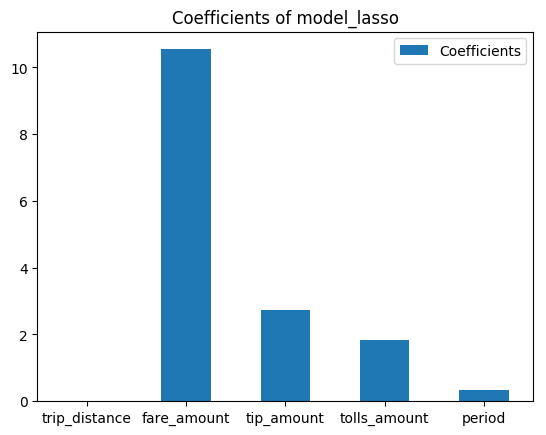
\includegraphics[width=0.7\textwidth]{plots/p13.png}
    % \includegraphics[width=\textwidth]{download.png}
    % this ensures your figures are centered where possible
    \caption{Lasso} % refer to this image as (Figure 1)
    \label{fig:image4}
\end{figure}


\subsection{Discussion}
As we can see of the three regression models, the fare\_amount features contribute to the final total\_amount most, since its coefficient is the biggest. We can indicate that the more fare\_amount the more total\_amount.

\section{Recommendations}
After all the analysis, we can learn that the weather affect the New York City taxi industry greatly. The colder the weather is the more people want to take taxi. But the cold day taxi trip distance is less than other season. In order for the taxi driver make more money the fare amount can take higher. 

\section{Conclusion}
All in all, by looking at the 2019 4 months and combine with New York City Weather Data 2019 data. We learn much more about the New York City taxi industry. The visualisation help us taxi usage on different weather. We also build model to predict the total amount. The fare\_amount affect the total\_amount the most.


\clearpage

% BEGIN REFERENCES SECTION
\printbibliography



\end{document}